\chapter{Odczytywanie losowego wyniku z kości}

\section{Przetwarzanie wstępne obrazów}

W niniejszym rozdziale omówiono proces przetwarzania wstępnego obrazów kości,
który przekształca dane pochodzące z fizycznego komponentu naszej maszyny (zdjęcia kości) na dane wejściowe dla modelu sztucznej inteligencji.
Przez dane wejściowe dla modelu SI rozumie się tutaj odpowiednio sformatowane obrazy, a więc takie w skali szarości,
o rozmiarach 64x64 piksele, zawierające jedynie kość wyciętą ze zdjęcia całego bębna maszyny.

\subsection{algorytm}

Przetwarzanie obrazów składa się z kilku etapów, które dokładnie opisano poniżej, a workflow prezentuje się tak:
1. Wczytanie obrazu wejściowy \\
2. Odnalezienie kości za pomocą maski na komponencie nasycenia \\
3. Stworzenie i wycięcie prostokąta "Bounding Box" wokół maski \\
4. Przeskalowanie do odpowiedniego rozmiaru \\
5. Konwersja do skali szarości \\
6. Zapisanie gotowego obrazu \\

Na rysunkach <NUMERY> przedstawiono przykładowe zdjęcie surowe oraz poddane już wstępnemu przetwarzaniu.

%% Czy np. dodać elementy pośrednie? - idk

\begin{figure}[H]
    \centering
    \begin{minipage}[t]{0.45\linewidth}
        \centering
        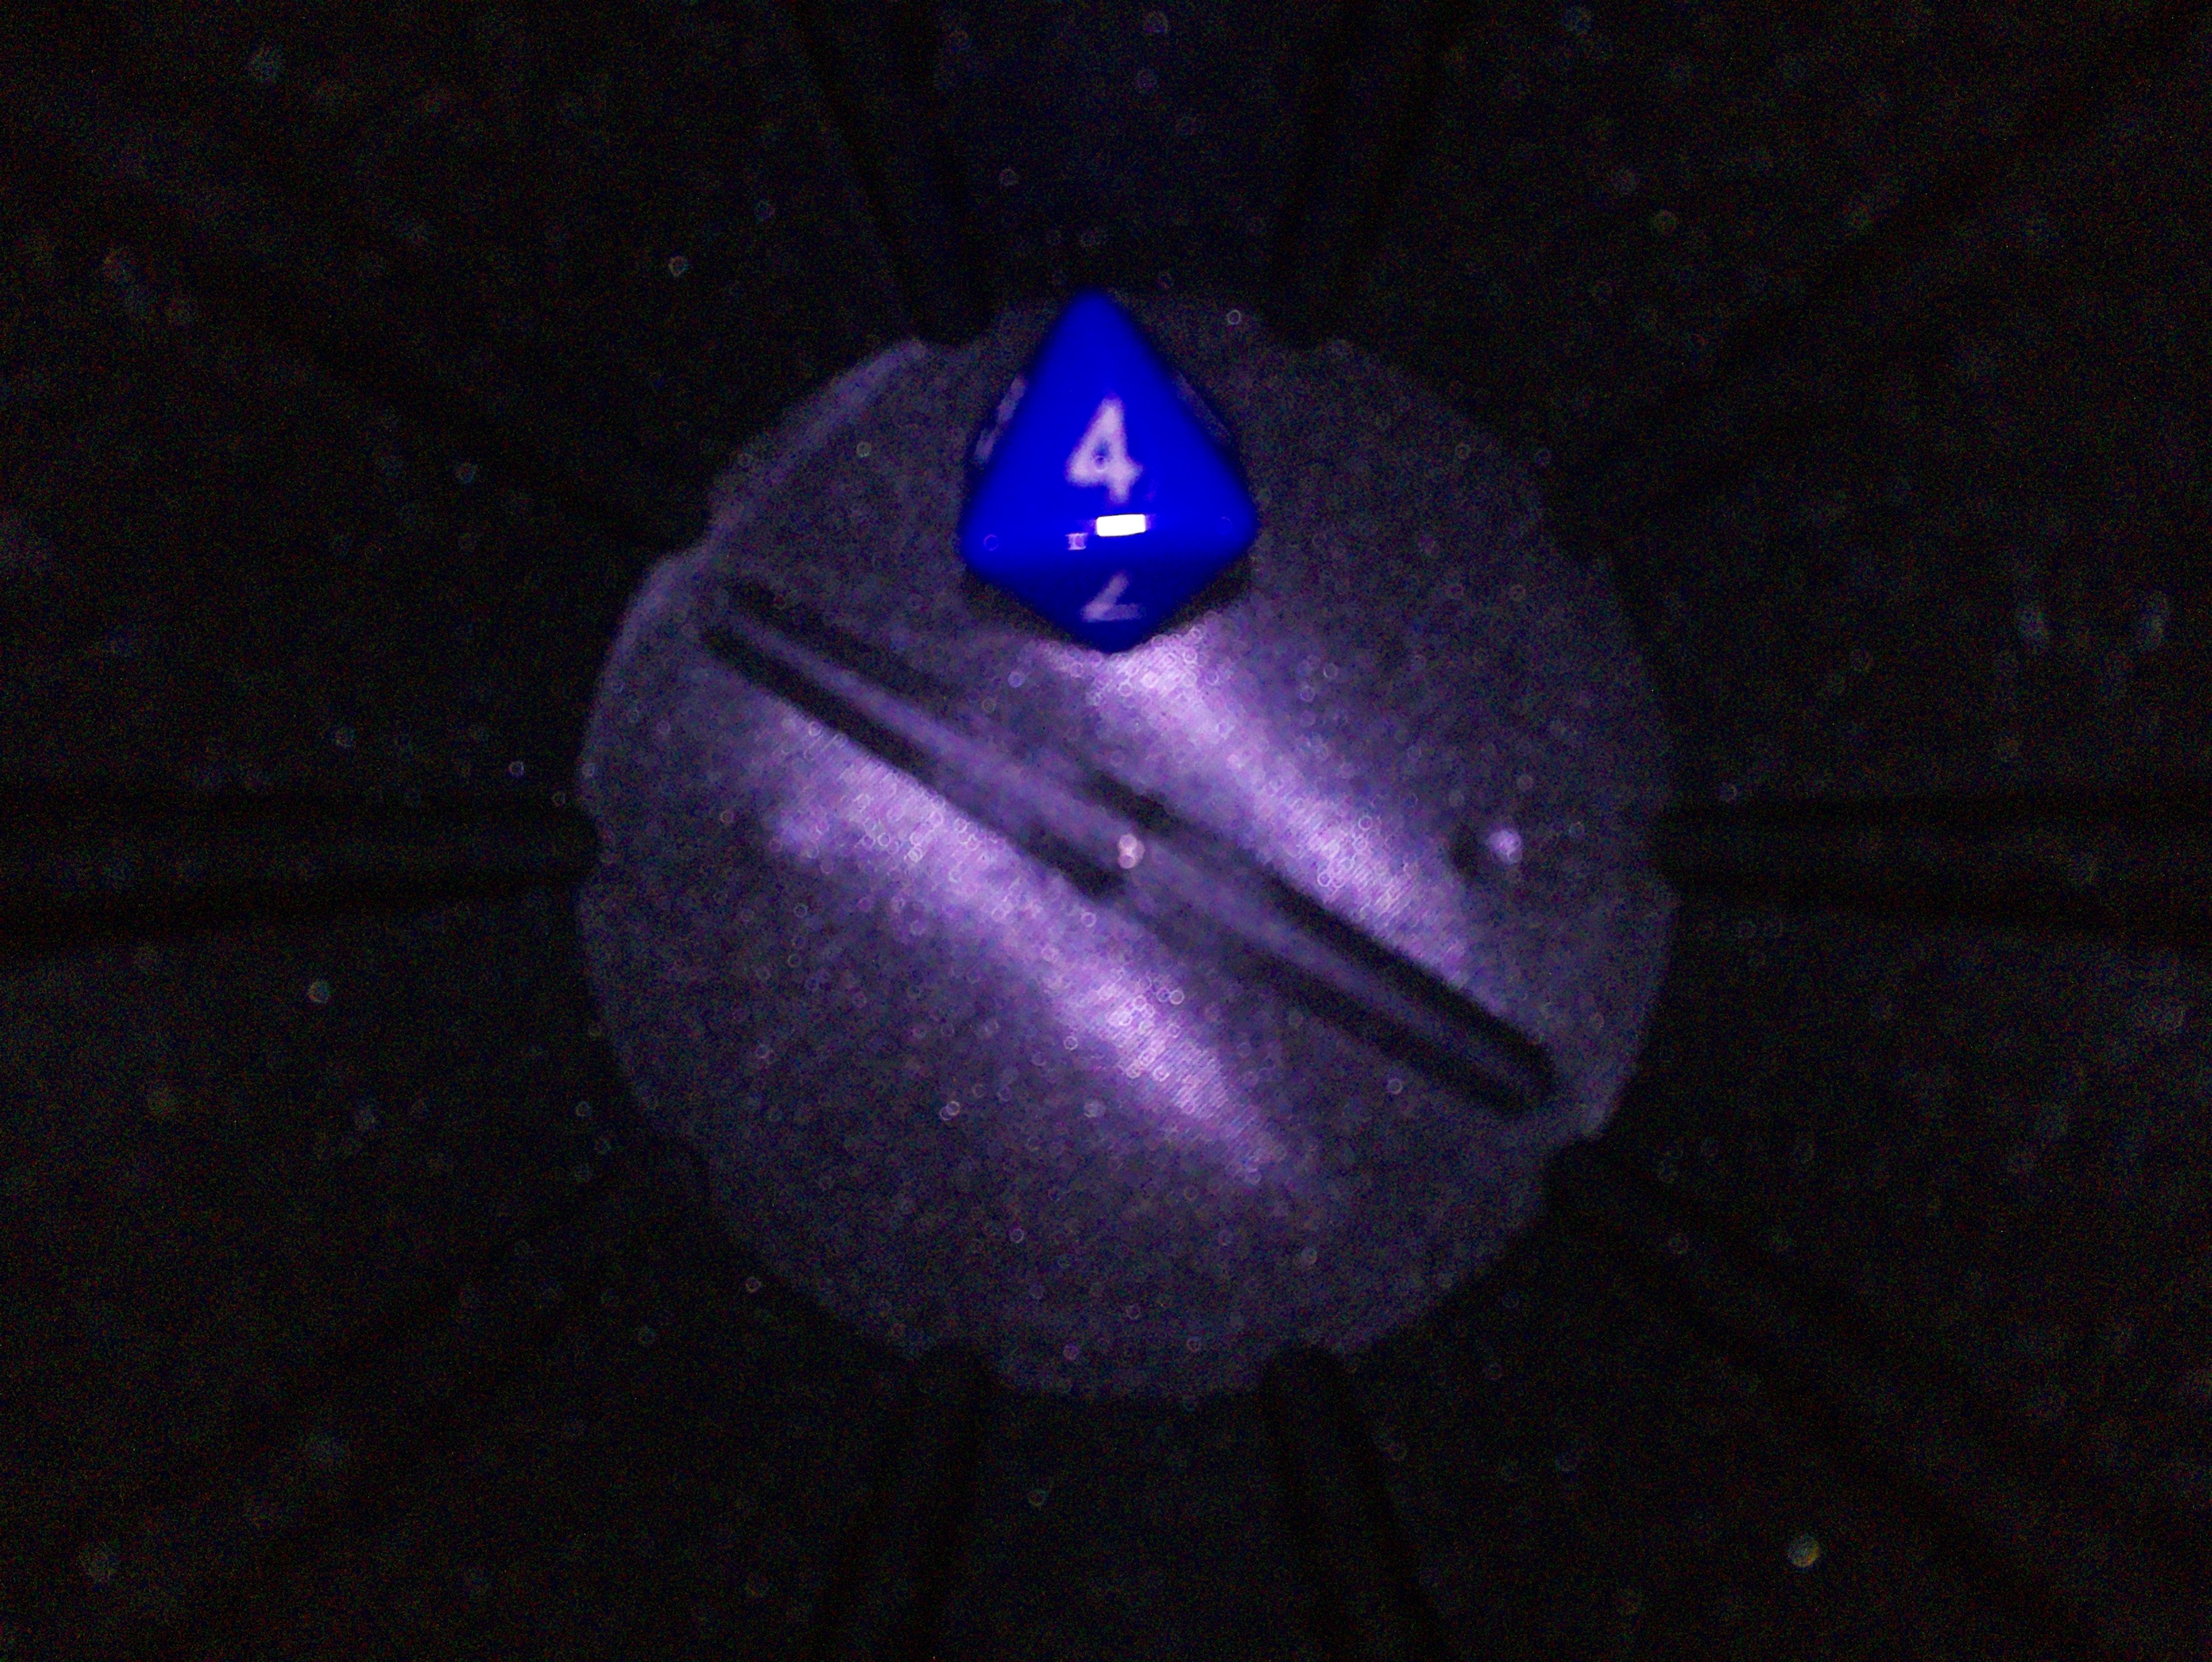
\includegraphics[width=\linewidth]{chapters/04-czytanie/figures/4raw}
        \caption{Surowe zdjęcie z kamery urządzenia}
        \label{fig:4raw}
    \end{minipage}
    \hfill
    \begin{minipage}[t]{0.45\linewidth}
        \centering
        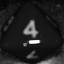
\includegraphics[width=\linewidth]{chapters/04-czytanie/figures/4processed}
        \caption{Zdjęcie poddane preprocessingowi}
        \label{fig:4proc}
    \end{minipage}
\end{figure}


Przedstawiony algorytm został zaimplementowany w języku Python, a jego zadaniem jest identyfikacja, wycięcie i przeskalowanie obszarów zawierających obiekty zainteresowania w zdjęciach.

Zdjęcia w formacie JPEG są wczytywane za pomocą biblioteki Pillow, a następnie konwertowane do przestrzeni kolorów RGB, co zapewnia jednolitość formatów danych wejściowych.

Obrazy są przekształcane do przestrzeni barw HSV, aby oddzielić komponenty odpowiadające za barwę (H), nasycenie (S) oraz jasność (V).
Nasycenie jest następnie wygładzane przy użyciu filtra Gaussa:

--- TODO ---
jakieś cytowanie, o tym czemu filtr Gaussa?

Na podstawie komponentu nasycenia (Saturation) oraz progowania tworzona jest maska binarna, która identyfikuje obszary o wysokim nasyceniu (a więc naszą kość).

W celu usunięcia niewielkich luk w masce binarnej stosowana jest operacja zamknięcia morfologicznego z wykorzystaniem strukturalnego elementu prostokątnego z zaimportowanego modułu cv2

TODO - cytowanie o zamknięciu morfologicznym?  \\

Maska jest analizowana w celu zlokalizowania największego konturu, który określa obszar zainteresowania.
Na tej podstawie oryginalny obraz jest kadrowany w kształt prostokąta wokół obszaru zainteresowania,
a następnie przeskalowywany do wymiarów $64 \times 64$ pikseli:

Ostatecznie obraz jest konwertowany do skali szarości, co redukuje wymiarowość danych
i umożliwia naszej sieci neuronowej skupienie się na strukturze obrazu.

Dodatkowo, konwersja do skali szarości pozwala znacznie lepiej poradzić sobie z problemem odblasków,
powstających gdy kość niefortunnie ułoży się pod takim kątem, że odbija światło którejś z diód wprost do kamery.

\subsection{Potencjalne trudności}

Wspomniane wcześniej odblaski znacznie pogarszają skuteczność odczytywania wyniku z kostki.
Jednak zastosowanie skali szarości pozwoliło w znacznym stopniu pozbyć się tego problemu, co pokazują rysunki 4.3 oraz 4.4.

\begin{figure}[H]
    \centering
    \begin{minipage}[t]{0.45\linewidth}
        \centering
        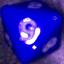
\includegraphics[width=\linewidth]{chapters/04-czytanie/figures/blask_raw}
        \caption{Odblask na przeskalowanym zdjęciu}
        \label{fig:blaskraw}
    \end{minipage}
    \hfill
    \begin{minipage}[t]{0.45\linewidth}
        \centering
        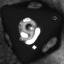
\includegraphics[width=\linewidth]{chapters/04-czytanie/figures/blask_proc}
        \caption{Odblask po zmianie na skalę szarości}
        \label{fig:blaskproc}
    \end{minipage}
\end{figure}

Inną trudnością, która objawiała się w początkowych fazach pracy były zupełnie czarne obrazy,
w wyniku problemu z działaniem diod, o czym więcej będzie powiedziane w rozdziale o problemach
--- TODO --- Tak zakładam, że to powinno być w innym, bo to sprzętowe i średnio tu pasuje, chyba (?)

Kolejną, znacznie częściej spotykaną trudnością w obecnej architekturze urządzenia są niejednoznaczne wyniki,
a więc moment gdy kość zatrzyma się w pozycji w której widać więcej niż jedną ściankę.
Najczęściej jest to spowodowane tym, że kostka zatrzymała się na śmigle napędowym, przez co wynik może być niejednoznaczny.
% TODO check nazwy śmigło!!! XD

\begin{figure}[H]
    \centering
    \begin{minipage}[t]{0.45\linewidth}
        \centering
        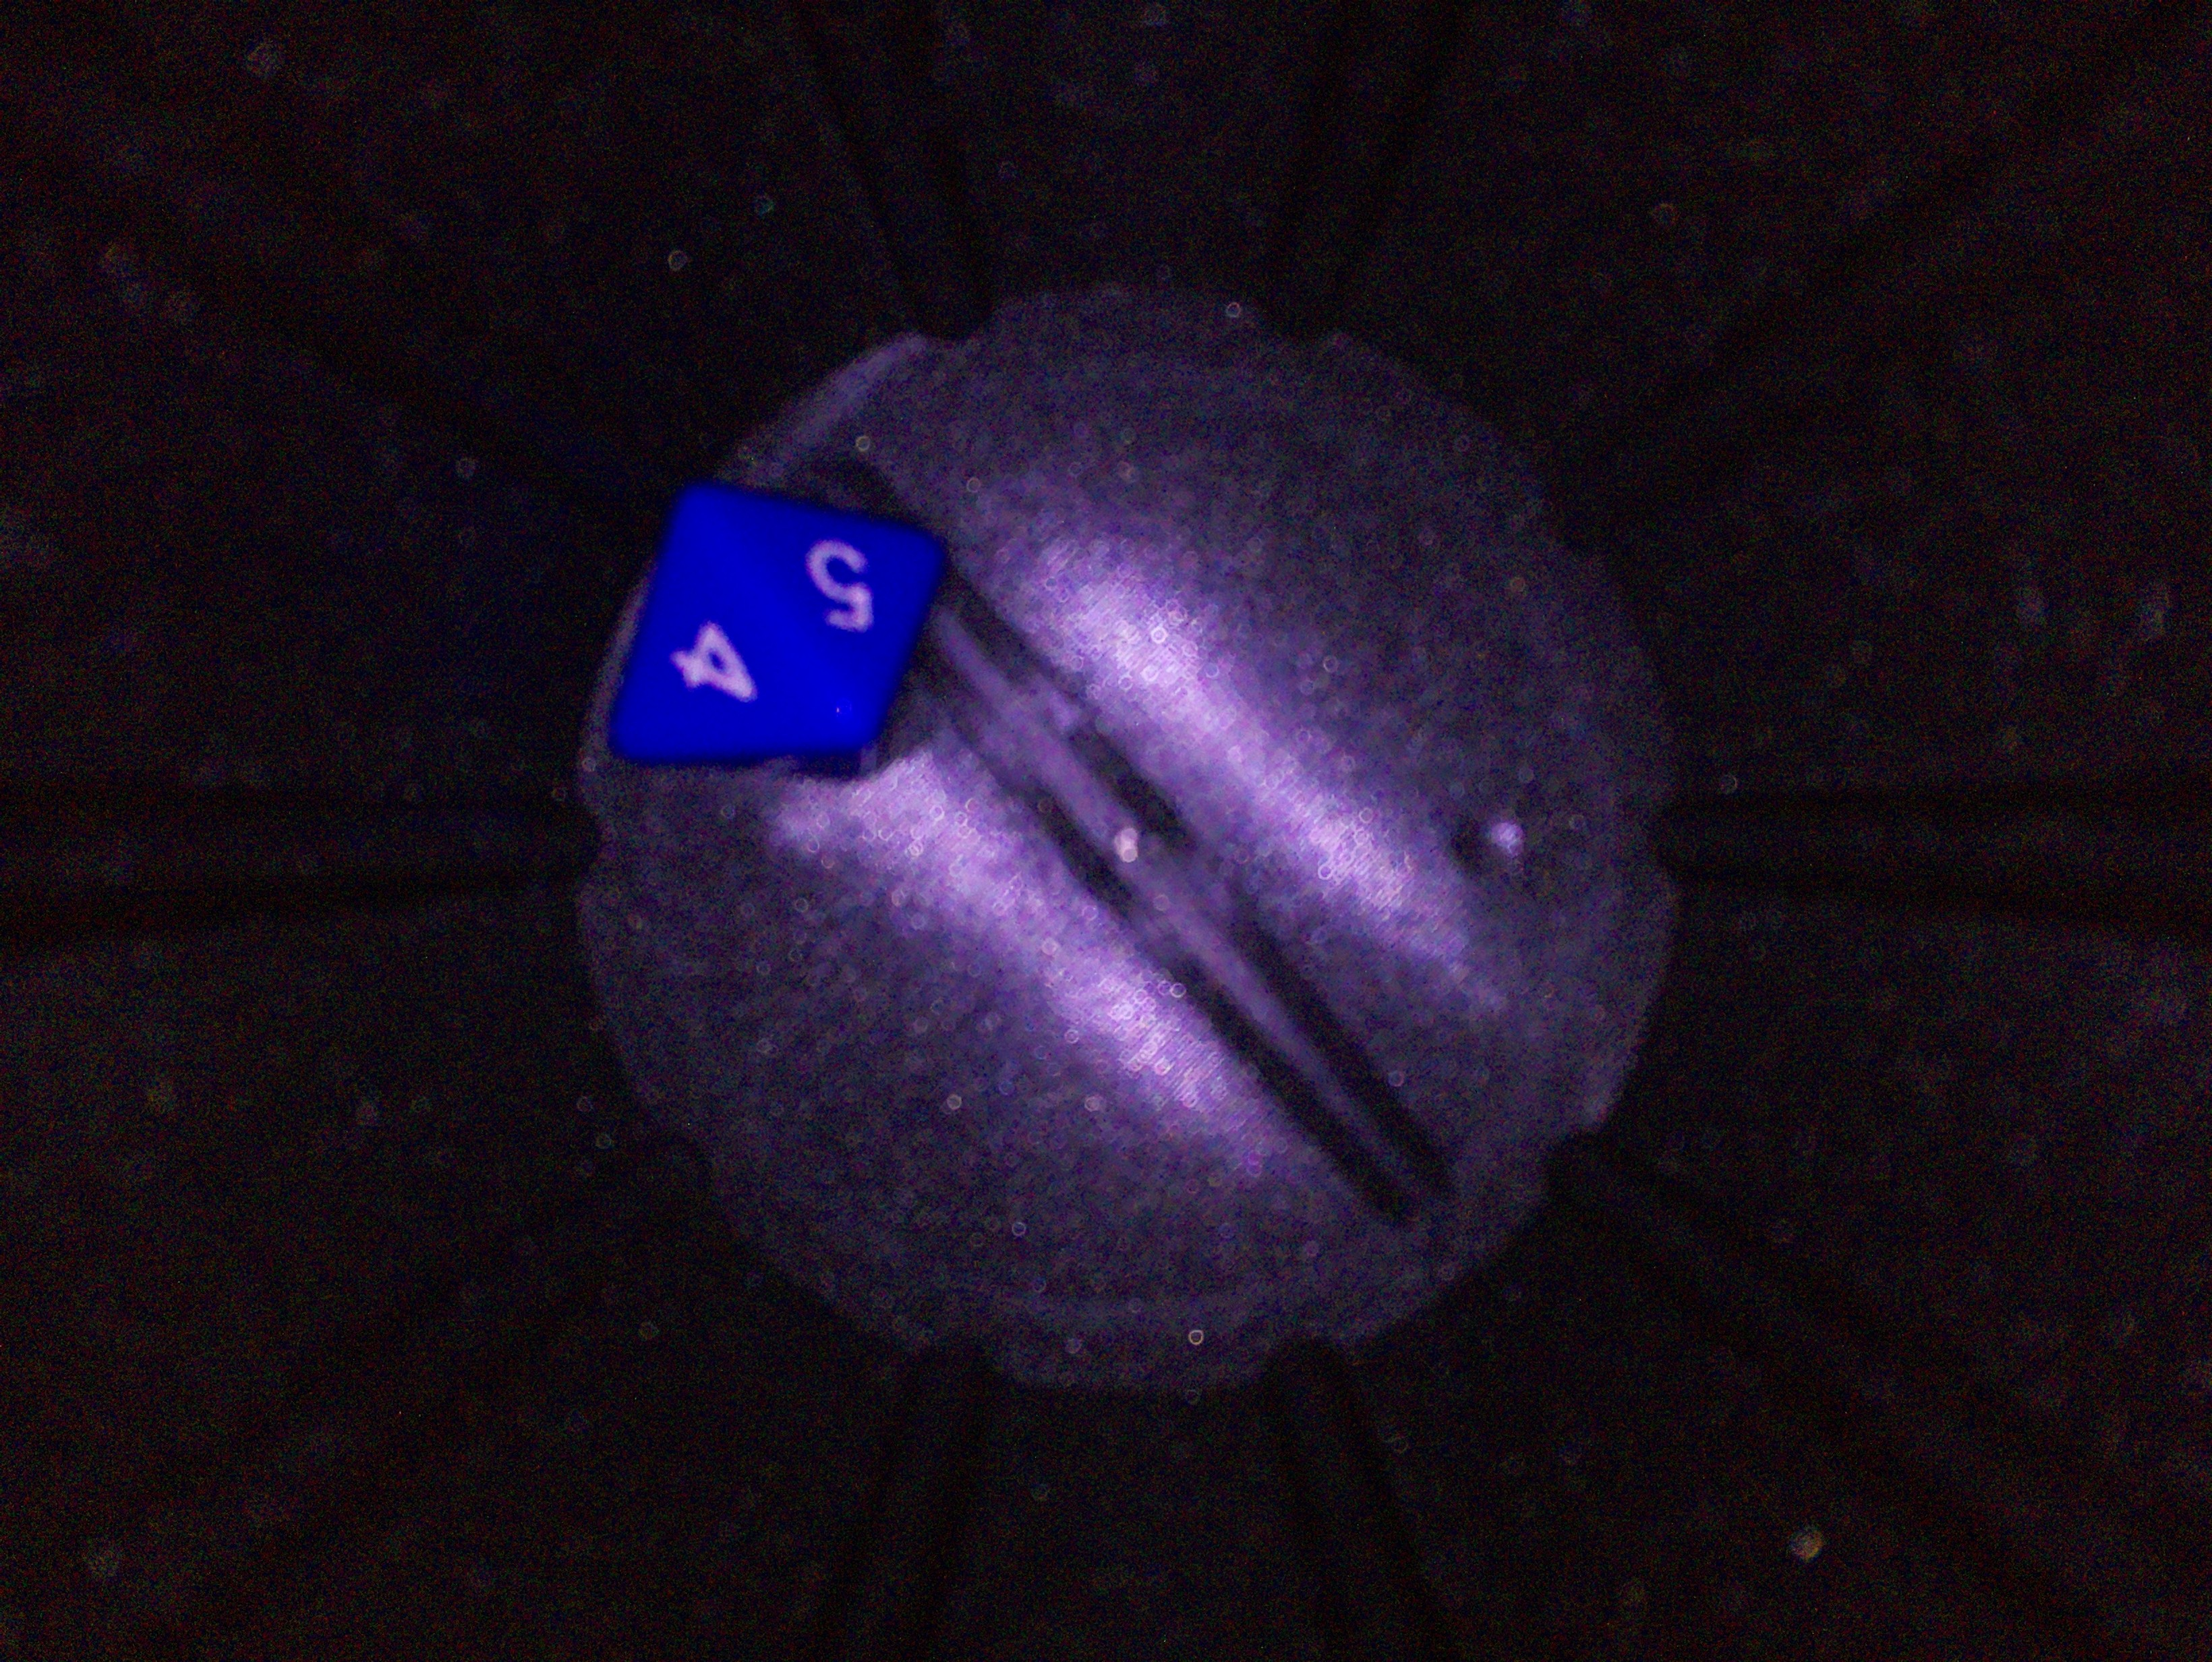
\includegraphics[width=\linewidth]{chapters/04-czytanie/figures/niepewne}
        \caption{Odblask na przeskalowanym zdjęciu}
        \label{fig:niepewne}
    \end{minipage}
    \hfill
    \begin{minipage}[t]{0.45\linewidth}
        \centering
        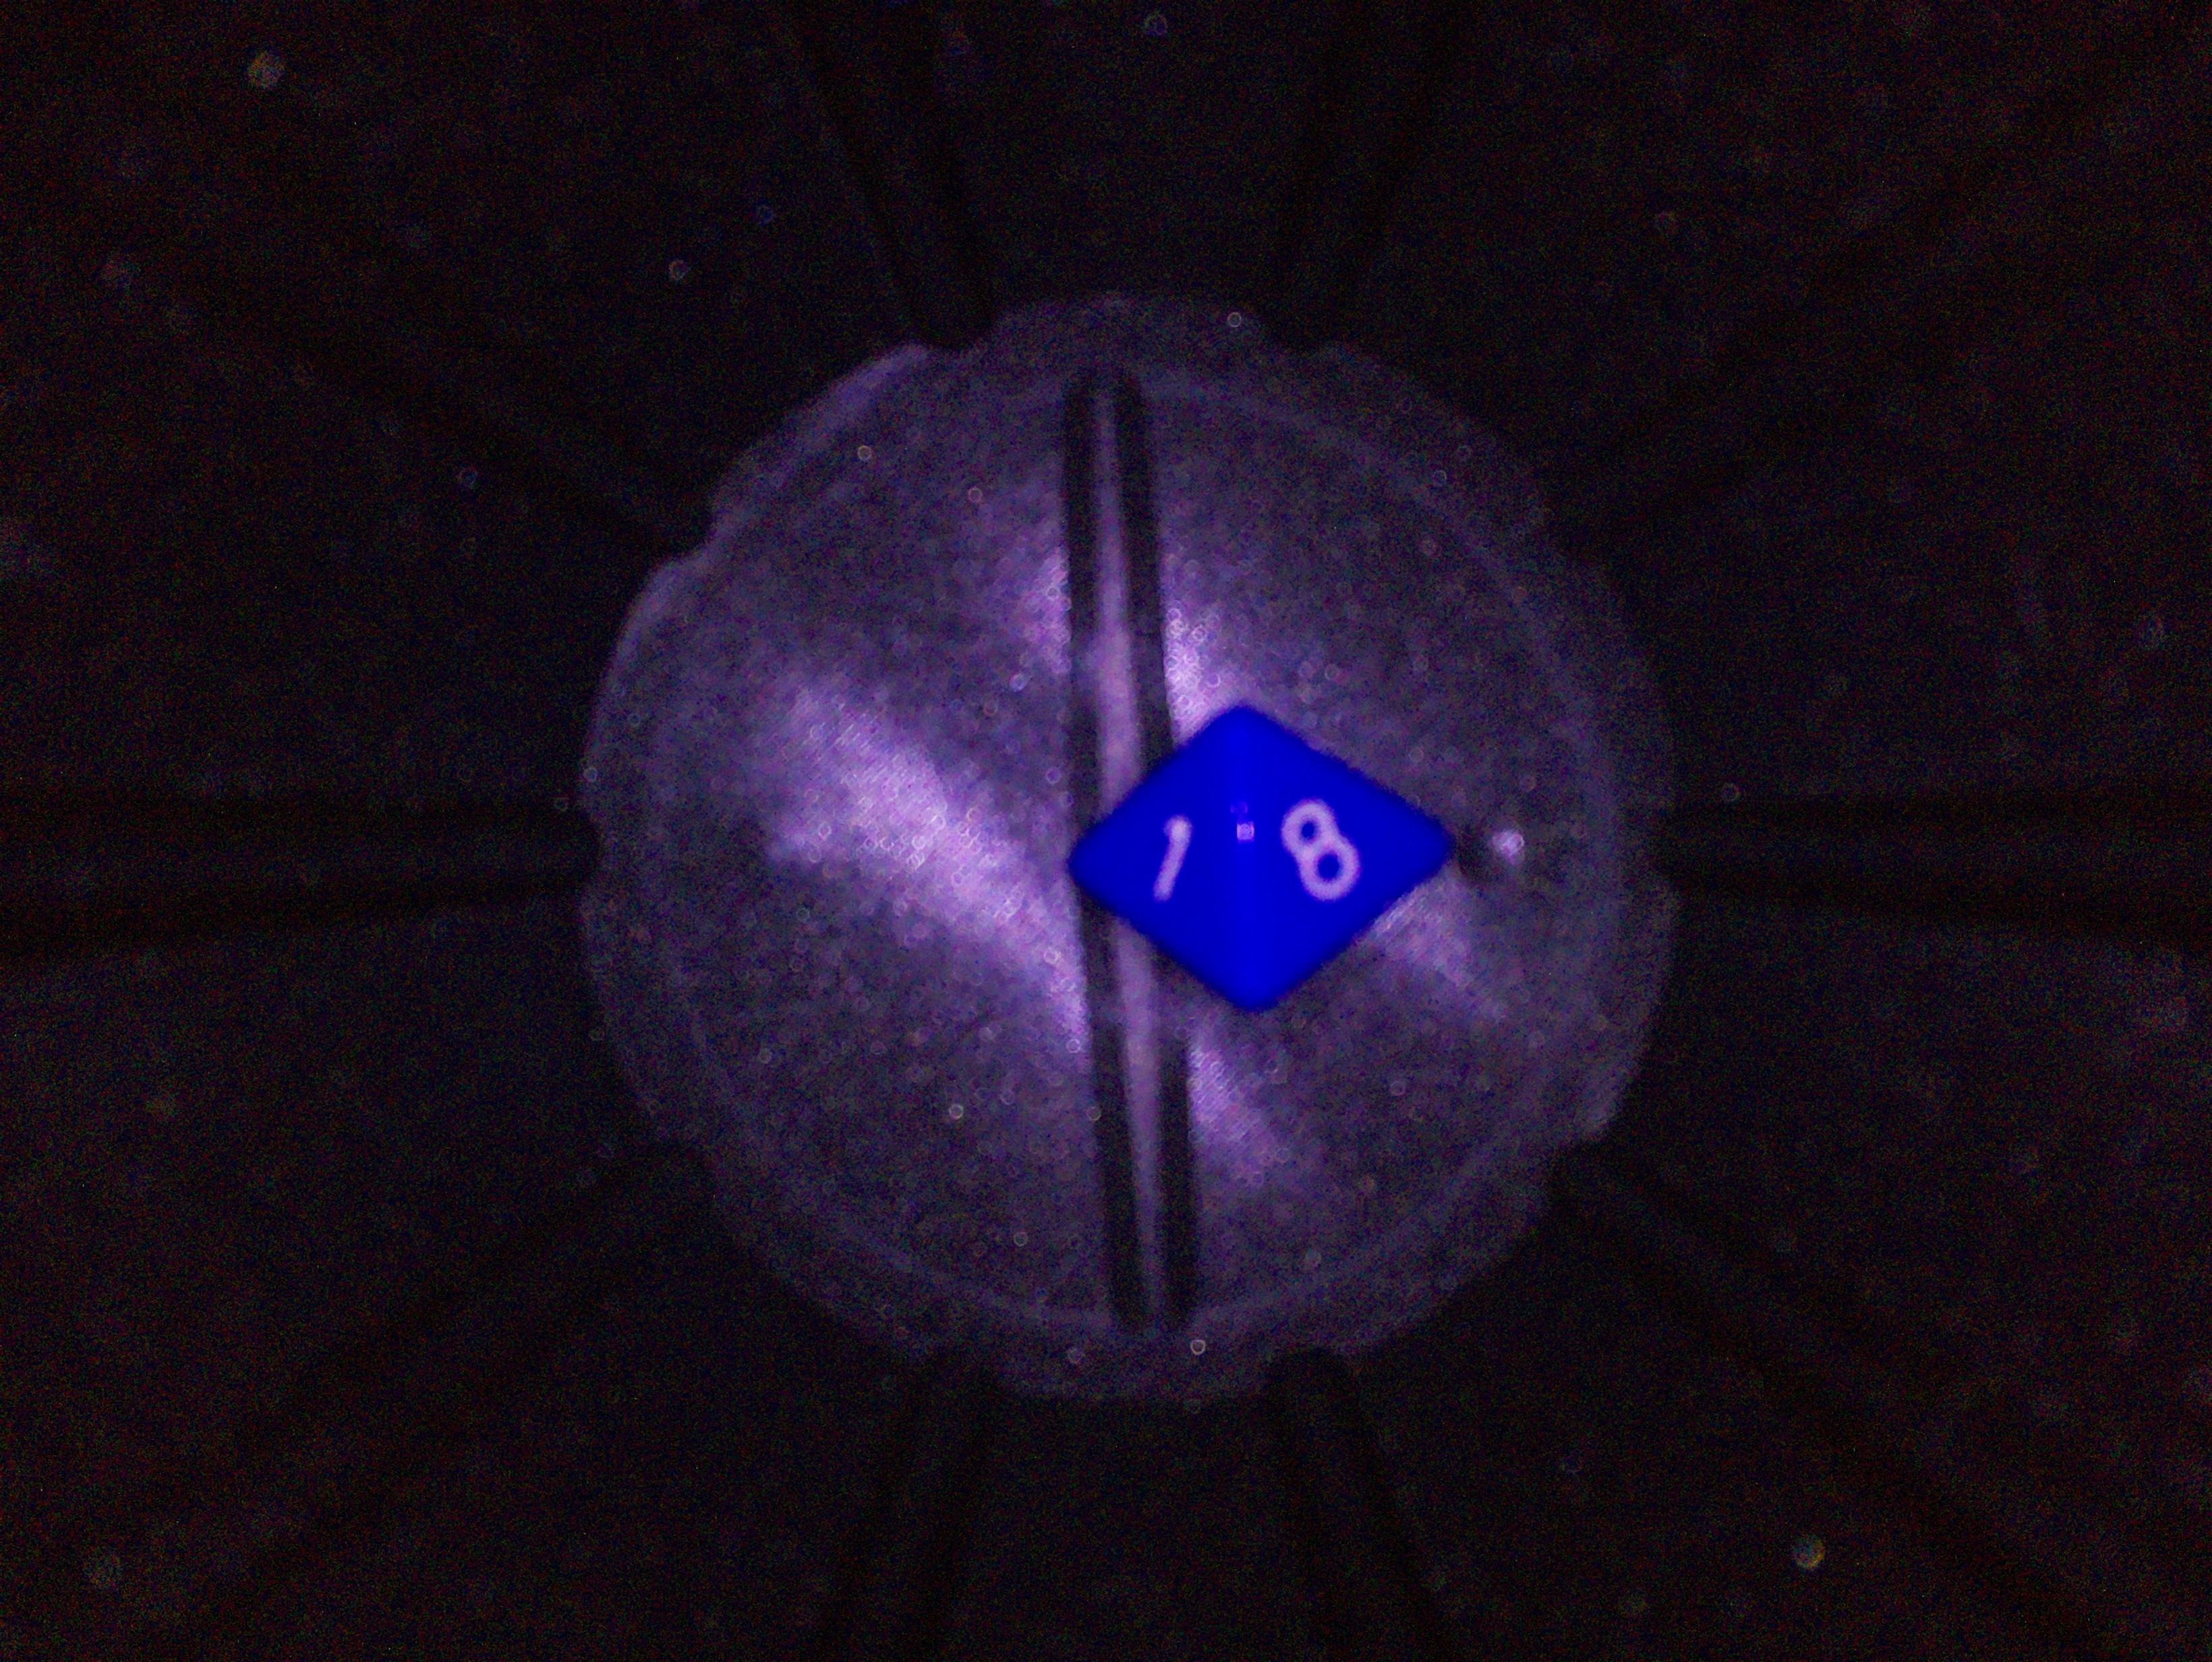
\includegraphics[width=\linewidth]{chapters/04-czytanie/figures/smiglo}
        \caption{Odblask po zmianie na skalę szarości}
        \label{fig:smiglo}
    \end{minipage}
\end{figure}

Rozwiązaniem tego problemu jest model dokonujący predykcji wyniku rzutu, który siłą rzeczy odczytuje ze zdjęcia tylko jeden wynik i wybiera ten,
który jest bardziej widoczny, ponieważ podczas uczenia został wyposażony również w takie niejednoznaczne sytuacje,
które byliśmy w stanie ręcznie oznaczyć właśnie na potrzeby nauczenia modelu.

Zdarzają się oczywiście rzadkie przypadki, w których kość wyląduje równo na śmigle, tak że wynik jest idealnie czytelny,
tak jakby wylądowała normalnie na podstawce kubka, ale wtedy problem z lądowaniem na śmigle nie istnieje,
gdyż nie przeszkadza to w tym że kość i tak zostanie podbita przy następnym obrocie śmigła.


Ostatnim rodzajem problemu jaki został napotkany był przypadek w którym kostka nie skończyła jeszcze swojej fazy lotu,
lub wpadła w bardzo długie wirowanie - efektywnie uniemożliwiając odczytanie wyniku.

\begin{figure}[H]
    \centering
    \begin{minipage}[t]{0.45\linewidth}
        \centering
        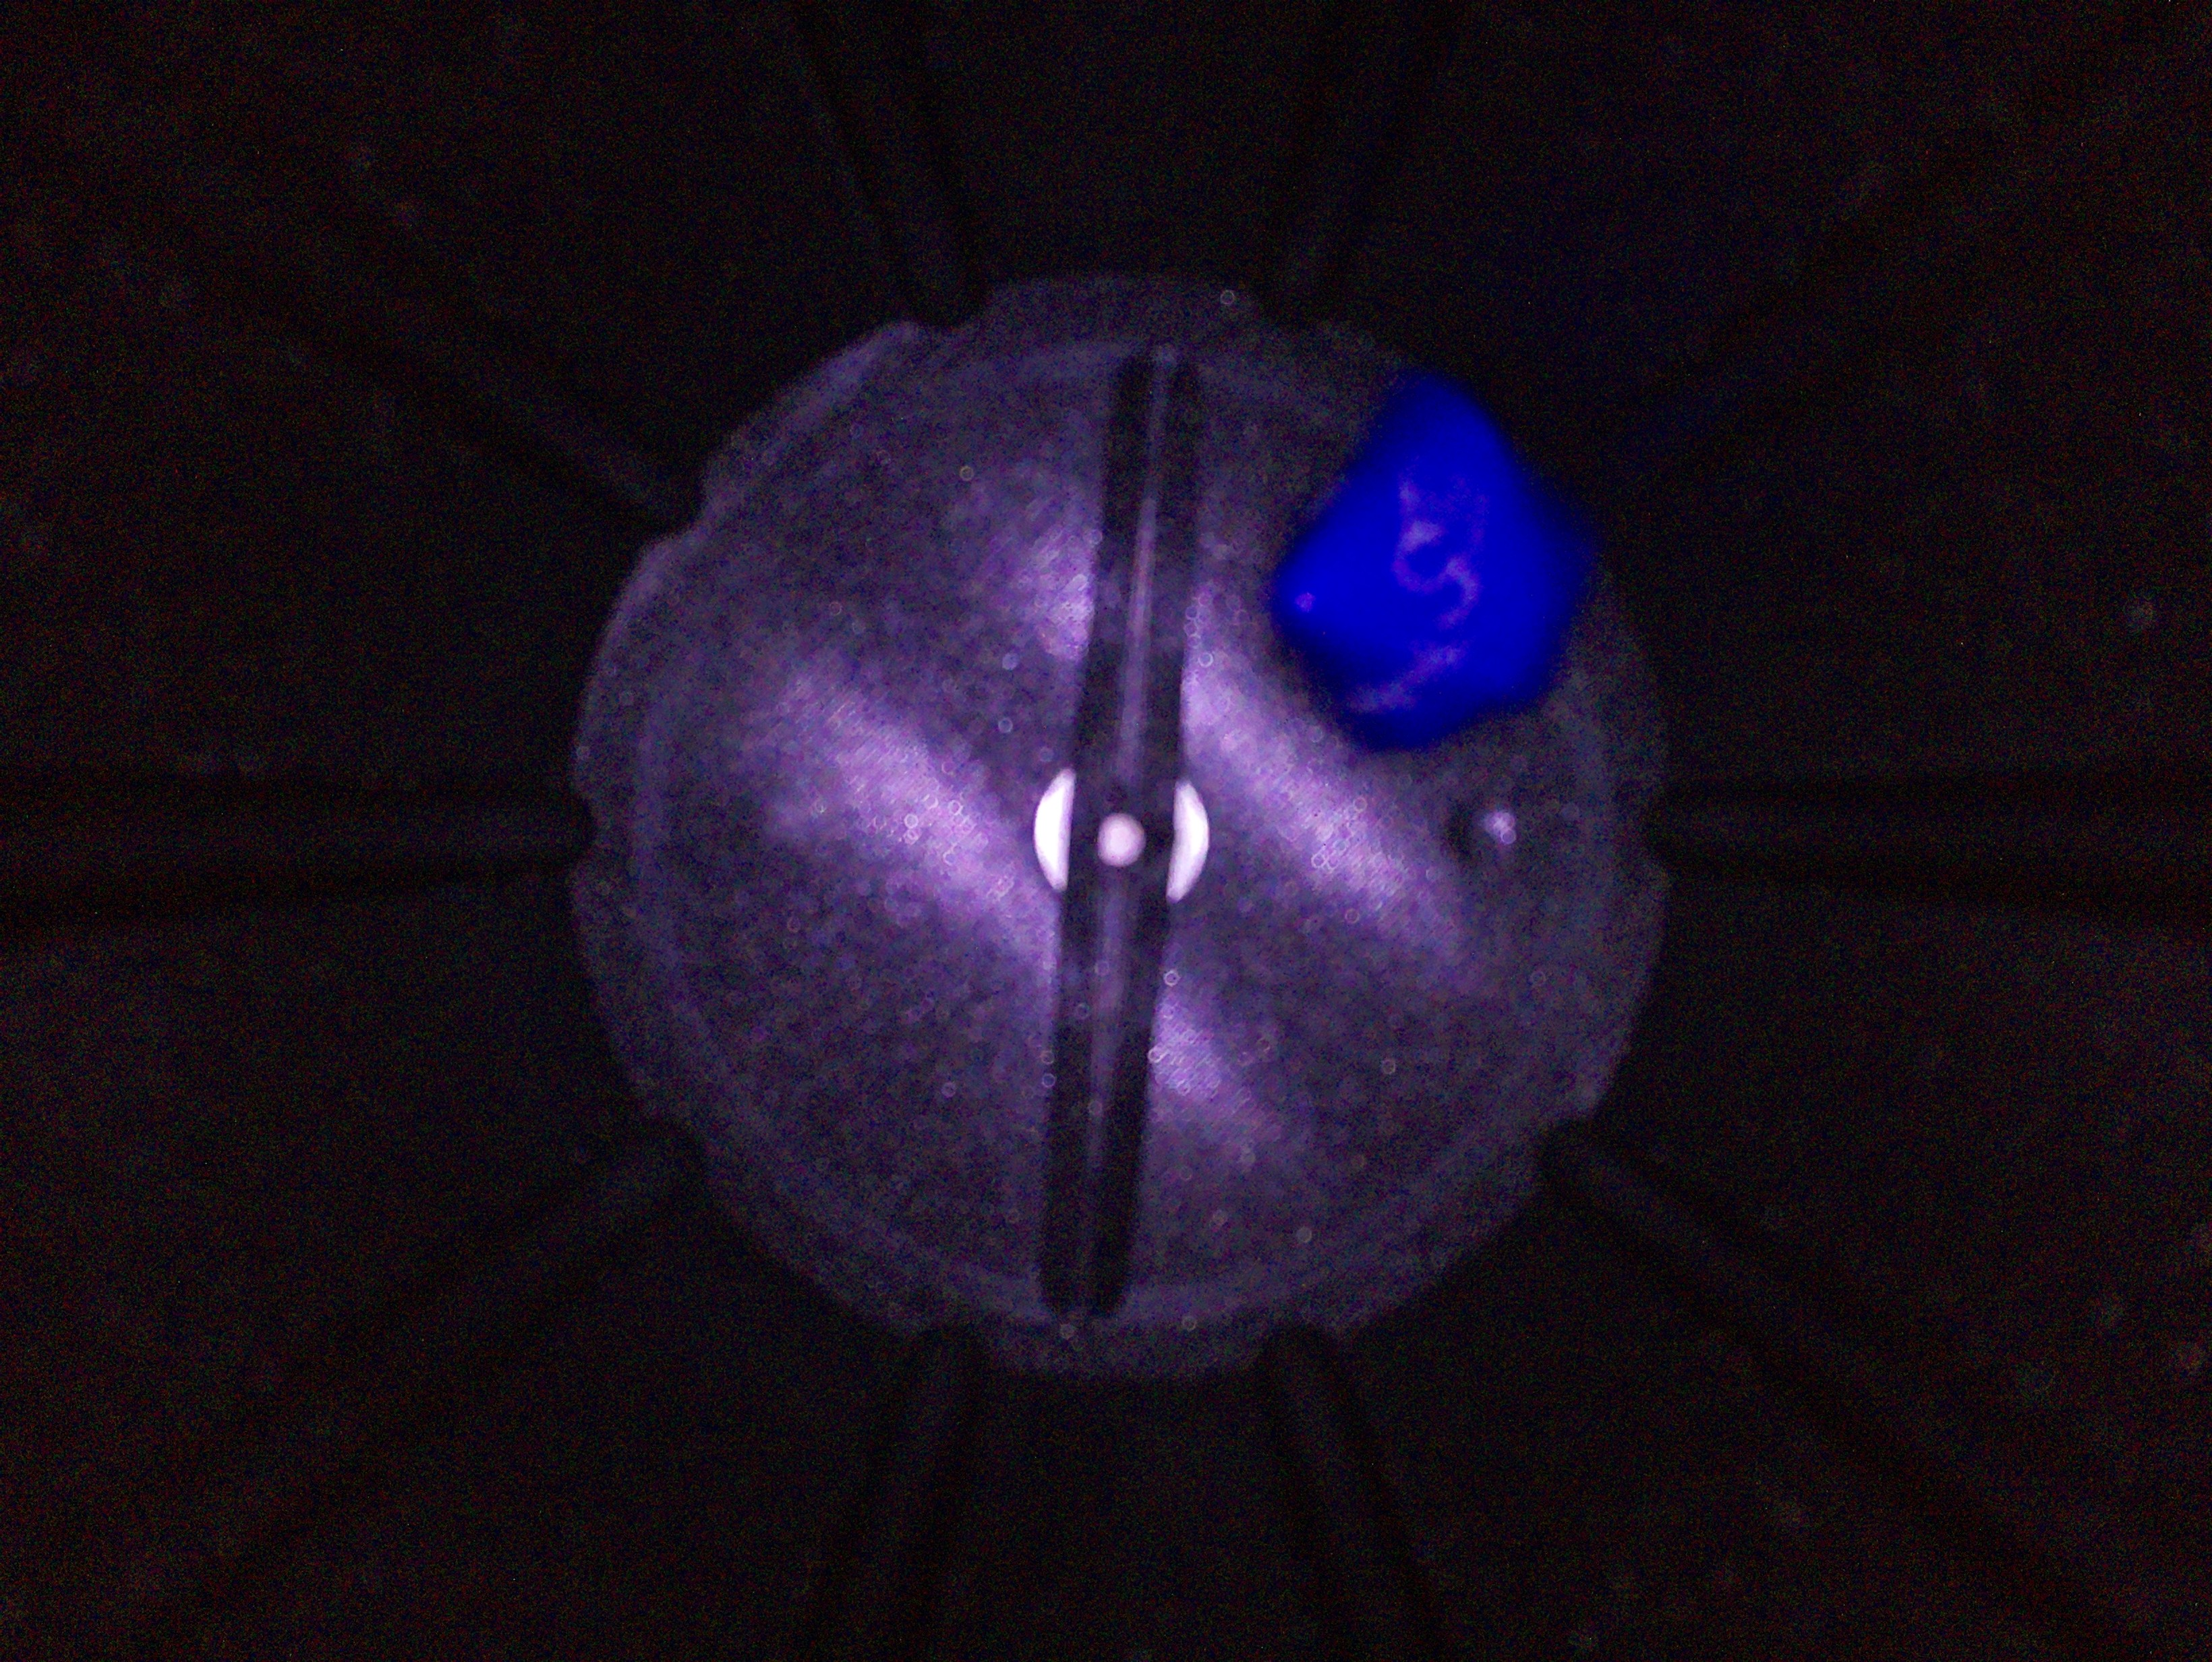
\includegraphics[width=\linewidth]{chapters/04-czytanie/figures/wir}
        \caption{Odblask na przeskalowanym zdjęciu}
        \label{fig:wir}
    \end{minipage}
    \hfill
    \begin{minipage}[t]{0.45\linewidth}
        \centering
        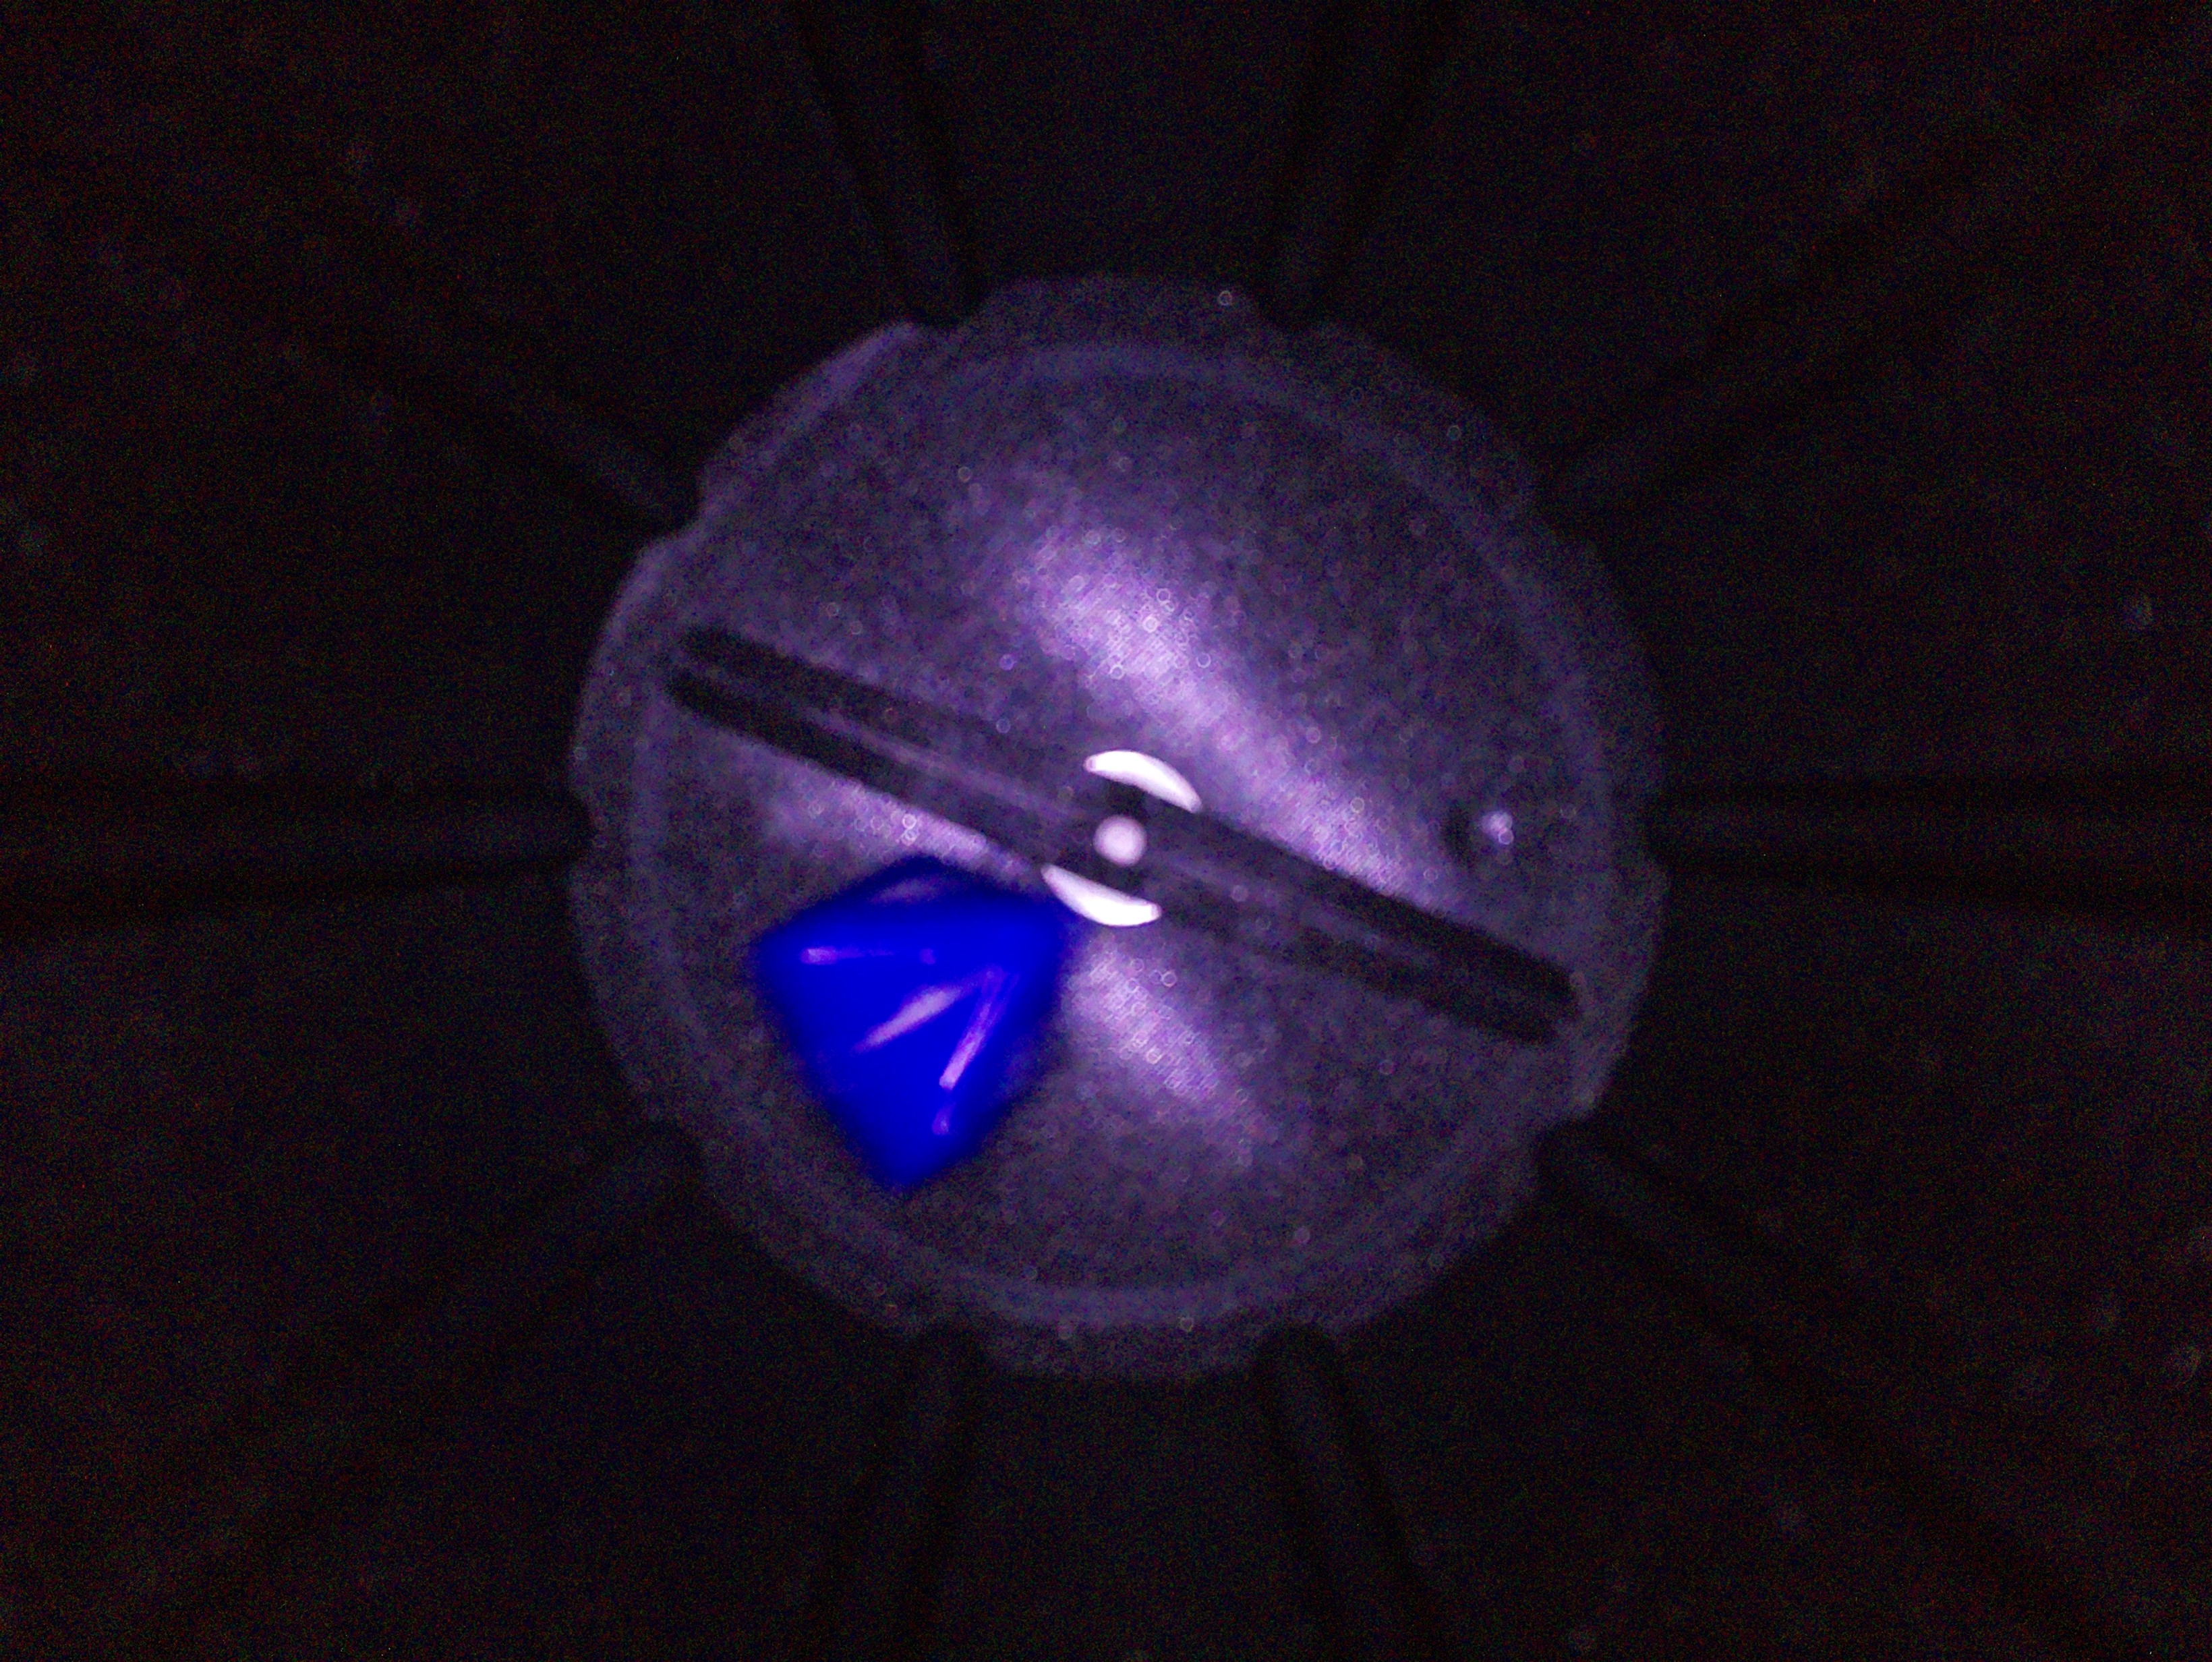
\includegraphics[width=\linewidth]{chapters/04-czytanie/figures/wir2}
        \caption{Odblask po zmianie na skalę szarości}
        \label{fig:wir2}
    \end{minipage}
\end{figure}

Rozwiązaniem większości wypadków w których zachodziła ta sytuacja okazało się spowolnienie działania maszyny.
Obecnie, oczekiwaniem aż kość zatrzyma się w miejscu steruje parametr czasowy, przyjmujący wartość jednej sekundy od zakończenia pracy śmigła.
Jest to wystarczające rozwiązanie, gdyż obecnie sytuacje niepewne z tego powodu zdarzają się bardzo rzadko (około 1 raz na 5000 rzutów).

Istnieje możliwość udoskonalenia tego rozwiązania, poprzez stosowanie detekcji ruchu kości,
jednak to rozwiązanie najpewniej okazałoby się bardziej kosztowne czasowo niż to proste czekanie stosowane obecnie.


--- TODO ---
jakoś to trzeba pewnie sprawdzić, bo nie mogę sobie tak gadać, nie?
Bo nie wiem, ale coś bym o tym pewnie napisał.



\section{Podsumowanie}

Przedstawiony algorytm przetwarzania wstępnego pozwala na skuteczne przygotowanie danych wejściowych dla modelu sztucznej inteligencji.
Automatyzuje proces identyfikacji i kadrowania obiektów zainteresowania w obrazach, co znacząco poprawia jakość danych.
Rozwiązanie zostało zaprojektowane z myślą o łatwej adaptacji do innych zastosowań wymagających podobnego przetwarzania obrazów,
dla przykładu przypadku zmiany kości w maszynie na inną, lub z inną ilością ścianek.

